\documentclass{article}
\usepackage[utf8]{inputenc}
\usepackage[parfill]{parskip}
\usepackage{graphicx}
\graphicspath{ {images/} }

\usepackage{subcaption}

\title{CS394R: Programming Assignment 2}
\author{Ashish Bora}
\date{September 2016}

\usepackage{hyperref}
\hypersetup{
    colorlinks=true,
    linkcolor=blue,
    filecolor=magenta,      
    urlcolor=cyan,
}

\begin{document}

\maketitle

\section{Introduction}

The gambler's problem is the following: You are a gambler. You have an initial capital of $x$, where x is an integer in the range $[1, n-1]$. At every step, you can bet an integer, non-zero amount of money. Whether you win or lose is determined by an independent coin toss which comes up heads with probability $p$. If the outcome is heads, you win an amount equal to your bet. If you lose, you lose all the money you bet. The game is over if the amount of money you have is either $0$ or greater than $n$. On finishing the game in any state greater $n$, a reward of $+1$  is given. Reward on all other transitions in $0$.

Your task is to maximize the expected reward by the end of the game. What should you do?

\section{Modeling using MDP}

This problem naturally fits in the Markov Decision Process (MDP) framework. The amount of money you have is the state. Actions are how much you bet. State transitions are stochastic and determined by outcome of a coin toss. The reward is $+1$ on reaching state $n$, and $0$ otherwise. $n$ and $0$ are absorbing states. The objective is to maximize the sum of undiscounted rewards till we reach one of the absorbing states.

Note that it never makes sense to bet more than $n/2$. If the current captial is $n/2 + x$, betting $n/2 - x$ is strictly better than betting anything greater than $n/2 - x$. This is because if we win the current bet, we reach $n$ in both cases, but if we lose, then having the bet $n/2-x$ leaves us with the most capital. Thus, combined with the monotonicity property we shall soon prove, considering action space for capital $x$ to be to be limited to $\left[1, 2, \cdots \min \left(x, n - x\right)\right]$ is sufficient.

\section{Optimal policy using value iteration}

We can use value iteration to solve this problem. Since the state space is fairly small, this can be done exactly.

We use $p = 0.4$ and $n = 100$. We perform experiments with two different initializations:
\begin{enumerate}
    \item Initial the state value for $n$ is $1$. For all other states, initial value is $0$.
    \item Initial the state value for $0$ is $0$. For all other states, initial value is $1$.
\end{enumerate}

\begin{figure*}
    \centering
    \begin{subfigure}[b]{\textwidth}
        \centering
        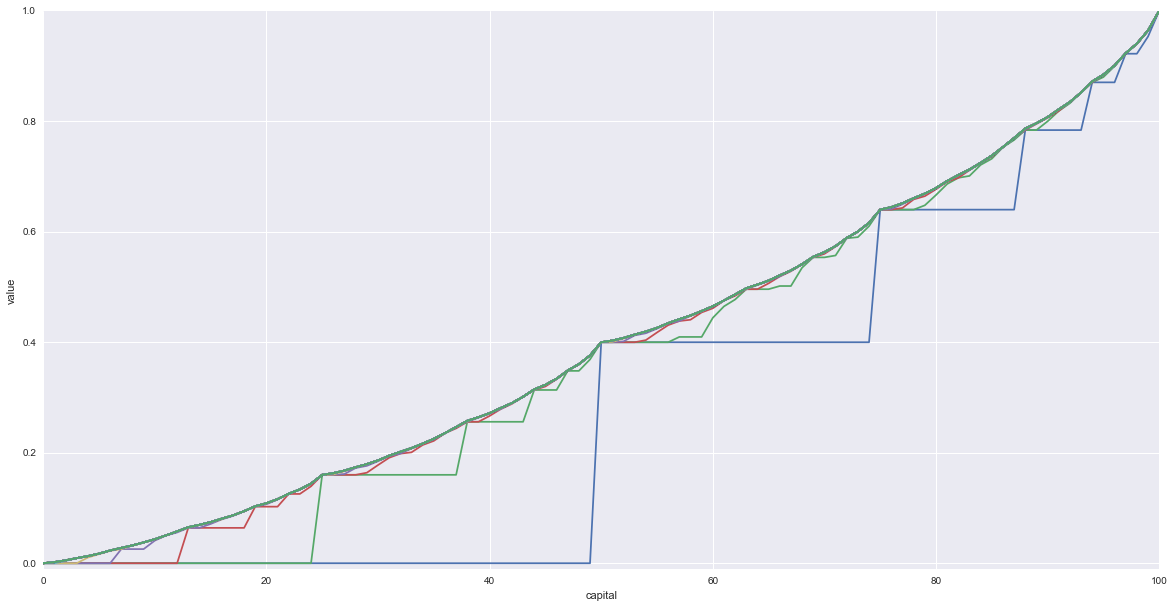
\includegraphics[width=\textwidth]{figure_1}
        \caption{Experiment 1}
    \end{subfigure}
    
    \begin{subfigure}[b]{\textwidth}
        \centering
        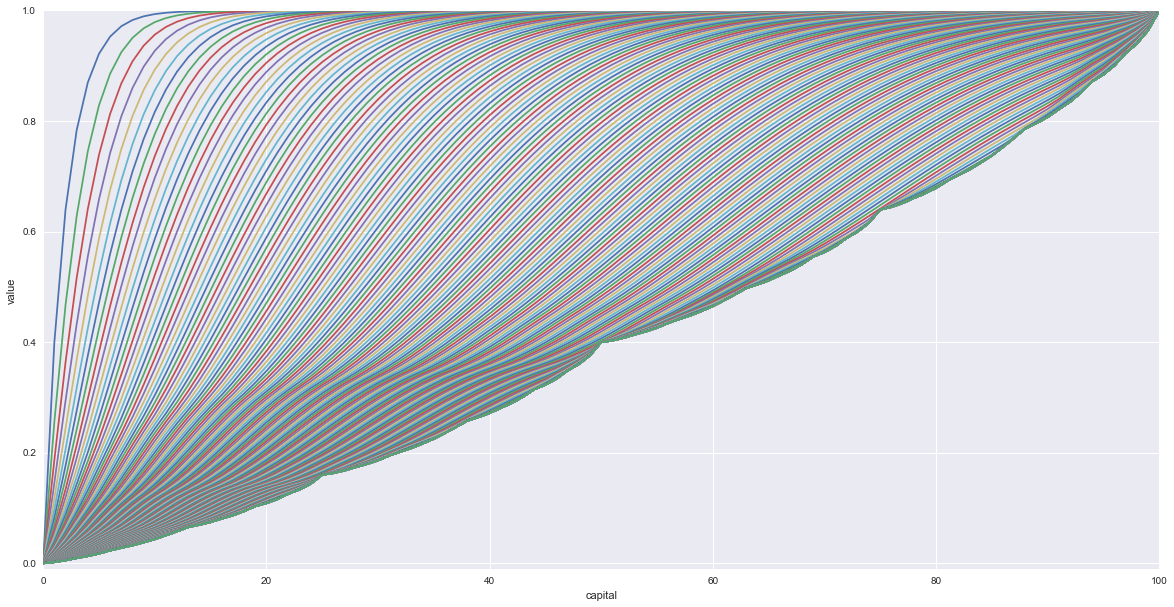
\includegraphics[width=\textwidth]{figure_4}
        \caption{Experiment 2}
    \end{subfigure}
    \caption{Value iterations}
    \label{value_iter}
\end{figure*}

The results plots of value vs state can be seen in Fig. \ref{value_iter}. Both experiments give identical value functions.

Thus, this experiment also empirically validates the theoretical result that the optimal value function is the unique fixed point of value iteration.

\section{Proof of monotonicity}

From Fig. \ref{value_iter}, we observe empirically that the optimal value function is monotonic. In this section we prove why this should hold for any $p$ and any $n$.

\textbf{Proof}

The reward is $+1$ if we reach $n$ and $0$ otherwise. Thus, the total reward is either $0$ or $1$. The expectation of total reward is thus, exactly equal to the probability of reaching $n$.


Let $\pi^*$ be the optimal policy. This means $V_{\pi^*}(x)$ = optimal probability of winning for starting capital $x$. Thus to prove monotonicity, we want to prove that $V_{\pi^*}(x) \leq V_{\pi^*}(x+1)$ for all $x$.

To prove this, it is sufficient to show that there exists a policy $\pi$ such that $V_{\pi}(x) = V_{\pi^*}(x)$ and $V_{\pi}(x) \leq V_{\pi}(x+1)$. Since $\pi^*$ is optimal, $V_{\pi}(x+1) \leq V_{\pi^*}(x+1)$, which would then imply $V_{\pi^*}(x) \leq V_{\pi^*}(x+1)$ as required.

One such (non-memoryless) $\pi$ is the following:
\begin{enumerate}
    \item If you start at any point other than $x+1$, follow $\pi^*$. This ensures that $V_{\pi}(x) = V_{\pi^*}(x)$.
    \item If you start at $x+1$, until you reach either $n$ or $x$, bet $min(y-x, y, n-y)$ where $y$ is your current capital. If you reach $x$, start following $\pi^*$. Thus, starting from $x+1$, following $\pi$, we will either reach $n$, or reach $x$ and win from there with probability $V_{\pi^*}(x)$. Thus, $V_{\pi^*}(x) \leq V_{\pi}(x+1)$.
\end{enumerate}

This completes the proof.

Note that we have implicitly used the fact that for any finite MDP, there exists a memoryless optimal policy. This is why $\pi^*$ will still dominate $\pi$, even though $\pi$ is non-memoryless.

\section{Optimal policies}

There are multiple known optimal policies for this task. These are shown in Fig. \ref{opt_policies}. Although no theretical analysis is known to prove that these are the only optimal policies, it can be easily checked that these policies are indeed optimal because they are fixed points with respect to the value function.

\begin{figure}
    \centering
    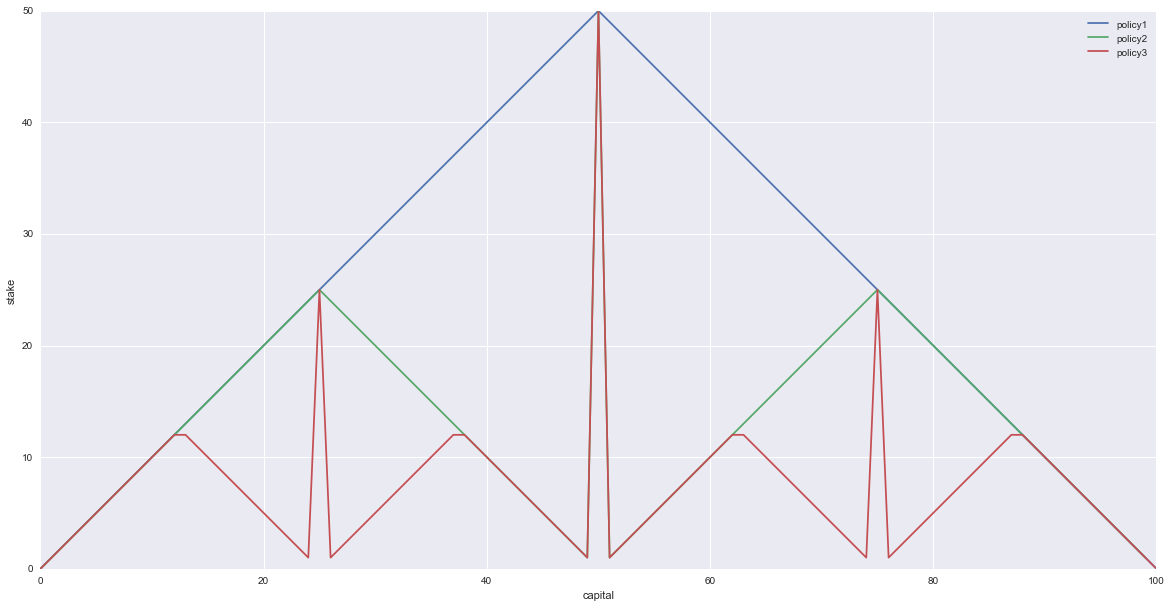
\includegraphics[width=\textwidth]{figure_3}
    \caption{Optimal Policies}
    \label{opt_policies}
\end{figure}


\section{Analysis of optimal policies}

As seen in Fig. \ref{opt_policies}, the optimal policies have quite interesting structure.

Policy1 (blue curve) is to bet $\min (x, n-x)$ starting at capital $x$. This has the following intuitive explanation -- since $p < 0.5$, the gambler has an incentive to minimize the number of rounds of betting. Thus the strategy which bets as much as possible and needed to reach $n$ is optimal.

It is less clear why Policy2 and Policy3 are optimal.

\subsection{Hypothesis}

One possible hypothesis is that the gambler sets some goalposts and is trying to bet such that even in worst case, it never goes below the goalpost it is currently ahead of.

For $n = 100$, for Policy3, there are three goalposts at $25$, $50$, and $75$. When at $51$, having passed the goalpost of $50$, the gambler bets $1$ so that even in the worst case, the loss will never take the gambler below $50$.

For $n = 100$, for Policy2, there is only one goalpost at $50$.

The next question we would like to investigate is how are these goalposts set? By observing the optimal policies, we can conjecture that the set of goalposts are $$\left\lbrace i\frac{n}{2^k} \ | \ i \in [1, 2^k-1] \right\rbrace$$ for some $k$ such that $n/2^k$ is an integer. Policy1, Policy2, and Policy3 have k equal to $0$, $1$, and $2$ respectively. 

What explains this structure of goalposts? The main idea I propose is that this is determined by the number of hops needed to reach $n$.

Consider the case with $n=100$. Lets say you start at $49$. No matter how smartly you play, you will need at least two hops to reach $100$. This suddenly changes if you start at $50$, since from there you can get to $100$ in one hop. This is the reason why $50$ is one of the goalposts. Same reasoning goes for $25$.

For $75$, the explanation is a bit more tricky. From $74$, you can reach $100$ in one step. But to do so you will have to bet $26$. Now if you lose that, you reach $48$, from where you will need two more hops to reach $100$. On the other hand, if you are at $75$, you need to bet $25$ to reach $100$. Now even if you lose, you are at $50$, and $100$ is reachable from there with one hop. Thus, there is a discontinuity in number of hops at $75$ which makes it another goalpost.

\subsection{Hypothesis test -- Steps to completion}

Reaching goalposts and trying to stay ahead of them leads to cautius play. i.e. when at $51$, with the goalpost of $50$, the gambler bets $1$ which is a very cautius bet.

If the goalpost hypothesis is correct, then more the number of goalposts, more cautius is the play and thus it will make more time to end the game. We can empirically test this by measuring how many steps it takes to reach the end of the game under different policies, starting at different initial capital.

\begin{figure}
    \centering
    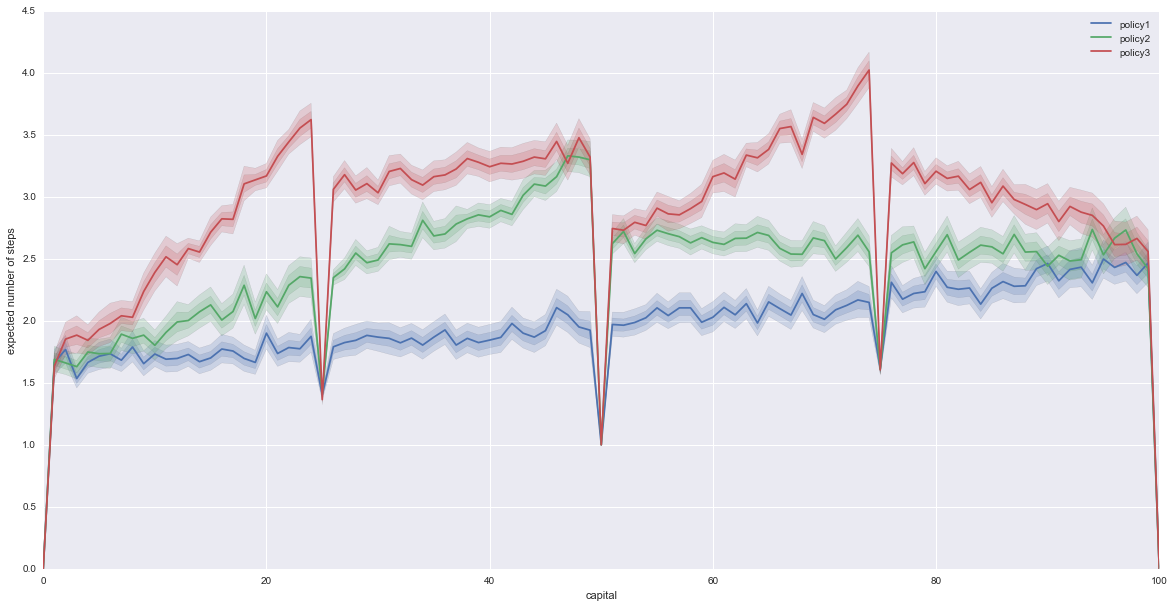
\includegraphics[width=\textwidth]{figure_2}
    \caption{Steps to completion}
    \label{steps}
\end{figure}

Fig. \ref{steps} shows the results of this experiment. On the x axis, we have the initial capital. On the y axis, we plot the number of steps needed to reach the end of the game under different policies. Each datapoint is estimated by 500 independent runs and we show the mean and $0.68$ and $0.95$ confidence intervals around each data point.

First, we observe that the number of steps needed is exactly the same for all 3 policies for initial capital values of $25$, $50$ and $75$. This is because from those values, all three policies are essentially equivalent as they hop between ${0, 25, 50, 75, 100}$ and have the same bets at all of these points.

Next, we observe that the policies with more goalposts, indeed require more steps to end the game. This is consistent with the view of cautious betting as described earlier.

\subsection{Hypothesis Test -- $\epsilon$ discouragement}

From Fig. \ref{steps}, we see a large gap between the number of steps to reach completion between the three policies. This hints that these are well separated in policy space.

Which of these policies are robust with respect to small changes in the environment? To test this, instead of giving $0$ reward, I tried to give a very small negative reward at every betting step. The final reward of +1 remains unchanged. With this new environment, which is arguably close to the original one, I tried to do value iteration and infer a policy based on the values.

Using $\epsilon = 10^{-10}$, I observed that the value graph looked almost identical. But Policy2 and Policy3 were no longer optimal. Policy1 continues to remain optimal. Since the new optimal policy is the same as the one of the old ones, the plot for number of steps will look exactly same as in Fig. \ref{steps}.

This means that the optimal policies may be highly discontinuous in terms of rewards and in particular, some optimal policies may even be destroyed by tiny changes to the reward function.

This is a repeated theme. For example, consider the problem of a reinforcement learning agent trying to learn to get out of a maze. If only a single positive reward is given at the end, many stupid policies are optimal, including random action policiy. But if we give a small negative reward at each timestep, most other optimas are destroyed and the one that remains is the one with minimal number of steps to destination.

PS: One physical analogy I thought of in this case is that of a water drops on a glass plate. If the plate is horizontal (think of slope of plate as rewards at intermediate time steps), all configurations of drops are stable -- in analogy to many optimas of the RL problem. But if you tilt the glass plate even slightly, almost all of them get destroyed leaving only a few that still remain optimal.

\section{Code and slides}
The code and slides used for presentation on this topic can be found \href{https://github.com/AshishBora/reinforcement-learning/tree/master/gamblers_problem}{here}.

\section{Conclusion}
In this assignment we defined the Gamler's problem, modeled it using MDP and solved it using value iteration. We then proved that the value function should be monotonic. We analyzed the optimal policies and while there is no known theoretical treatment, we proposed several hypothesis to explain the structure of the known optimal policies. We tested these hypothesis, and present a surprising result of optimas getting destroyed by miniscule changes to the reward function. Finally, we present several analogies to better understand this result.

\end{document}